\chapter{Work Instrumentation} \label{chap:instr}

In this section we describe how the computation of the work-metric can be performed during runtime by means of instrumenting the code.
In particular, we adapt the optimal algorithm proposed originally for profiling block frequency~\citep{nahapetian73,knuth73,ball94}.
Afterwards, we propose a relaxed instrumentation that focus on further reducing the overhead by considering the trade-off between profiling accuracy and instrumentation overhead.

Because we define work as a linear equation on the block frequency counters, it is possible to embed its computation into the execution of the program.
A naive instrumentation would consist basically of having a global counter that starts with the interception value, $\varepsilon$, and each basic block increments its own cost into the global counter.
Although this instrumentation is easily implemented, it imposes a large overhead on the instrumented program.
However, it is possible to insert fewer probes by carefully placing the probes in a way that is possible to reconstruct the complete profiling information~\cite{knuth73,ball94}.

\begin{figure}[h]
  \centering
  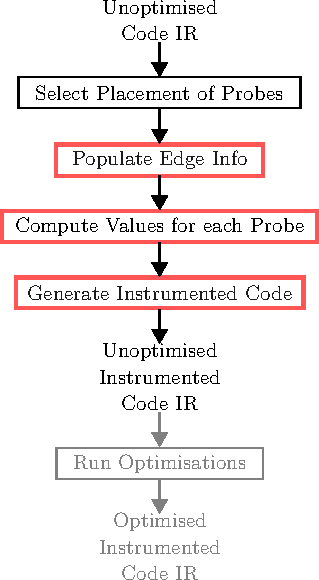
\includegraphics[scale=0.9]{figs/instr-diagram.pdf}
  \caption{Overview of the work instrumentation algorithm.}
  \label{fig:instr-diagram}
\end{figure}

We adapt the optimal block frequency instrumentation in order to perform the work profiling efficiently.
The proposed work instrumentation differs from the optimal block frequency instrumentation as the latter occurs in two stages:
\textit{(i.) Before execution.} The code is instrumented with counters for each probe.
\textit{(ii.) After execution.} The information from the recorded probes is propagated in the CFGs of the program.
In contrast, the work instrumentation has a single counter and it only requires the instrumentation before execution, without any post-processing of the recorded profiling.

Figure~\ref{fig:instr-diagram} shows a high-level overview of the complete work instrumentation algorithm.
The highlighted sections are introduced or improved by our work profiling  instrumentation.
The instrumented code is assumed to be generated before optimising the code.
This assumption is based on three key points:
\textit{(i.)} it guarantees that the work metric is independent of optimisation, i.e., the same input is always mapped to the same amount of work, regardless of the optimisation;
\textit{(ii.)} it simplifies the code generator;
\textit{(iii.)} it leverages from the optimisations to further improve the instrumentation code.
Having a work metric that is independent of optimisation is the most important reason for which we instrument the code before optimisations.

The optimal placement of the probes works exactly as previously described in Section \ref{subsec:optimalInstrumentation}.
It first computes the maximum spanning tree based on a weighing that assigns a non-negative value to each edge in the CFG.
These weights can be obtained either by empirical measurements or heuristic estimations, and their goal is to avoid probing in frequently executed edges.
Once we have the maximum spanning tree, probes are placed on every edge not in the spanning tree.
Figure~\ref{fig:cfg-example} shows an example of a CFG with a maximum spanning tree represented by the black edges, while the edges highlighted in red represent the placement of the probes.

\begin{figure}[htb]
\centering {
  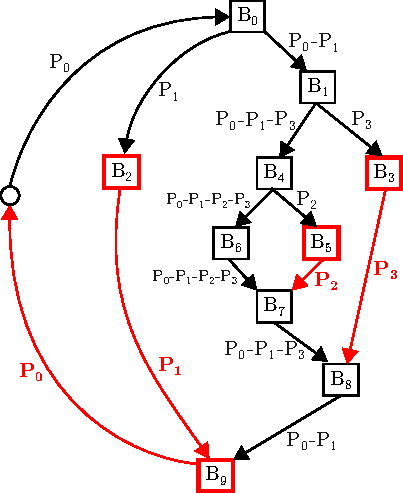
\includegraphics[scale=1]{figs/cfg-example.pdf}\\\vspace{1ex}
  \resizebox{0.8\textwidth}{!}{
  %\scalebox{0.8}{
     \begin{minipage}{0.5\textwidth}
     Instrumented value for each probe $P_i$:
     \begin{align*}
     w(P_0) &= w(B_0) + w(B_1) + w(B_4) + w(B_6) + w(B_7) + w(B_8) + w(B_9)\\
     w(P_1) &= w(B_2) - w(B_1) - w(B_4) - w(B_6) - w(B_7) - w(B_8)\\
     w(P_2) &= w(B_5) - w(B_6)\\
     w(P_3) &= w(B_3) - w(B_4) - w(B_6) - w(B_7)
     \end{align*}
     \end{minipage}
  }
}
  \caption{Example of a CFG with its minimum spanning tree in black and the
   basic blocks highlighted in red represent the instrumented basic blocks with
   the placement of the probes.}
  \label{fig:cfg-example}
\end{figure}

In contrast to the naive instrumentation where each basic block records only its own amount of work, with the optimal profiling, the instrumented basic blocks need to record an aggregated value of work that represents a path in the CFG.
These values are constructed with some instrumented basic blocks speculatively assuming some paths while other probes correct when these assumptions are wrong (see for example $w(P_0)$ and $w(P_1)$ in Figure~\ref{fig:cfg-example}).

%\begin{algorithm}[h]
%  \caption{Pseudocode of the data-flow analysis for assigning the values computed
%  in each probe of the instrumentation for the profiling of the work metric.}
%  \label{alg:populateEdgeInfo}
%  \begin{algorithmic}
%    \Function{\textrm{populateEdgeInfo}}{$G$}
%    
%    \For{\textbf{each} $e \in $ \textrm{instrumentedEdges}($G$) }
%       \State $B_I \gets $ \textrm{instrumentedBlock}($e$)
%       \State $inc[e] \gets \{ B_I \}$
%       \State $dec[e] \gets \{ \}$
%       \State $known[e] \gets $ \textbf{true}
%    \EndFor
%
%    \State $changed \gets $ \textbf{true}
%    \While{$changed$}
%       \State $changed \gets $ \textbf{false}
%	   \For{\textbf{each} $B \in V(G)$}
%          \State $uIn \gets $ \textrm{unknownIn}($known, G, B$)
%          \State $uOut \gets $ \textrm{unknownOut}($known, G, B$)
%		  \If{$uIn=0$ \textbf{and} $uOut=1$}
%             \State $changed \gets $ \textbf{true}
%		     \State $incOut \gets \{\}$
%			 \State $decOut \gets \{\}$
%		     \For{$B_p\in$ \textrm{predecessors}($G, B$)}
%			    \State $incOut \gets incOut \bigcup inc[(B_p,B)]$
%			    \State $decOut \gets decOut \bigcup dec[(B_p,B)]$
%			 \EndFor
%		     \For{$B_s\in$ \textrm{successors}($G, B$)}
%			    \State $incOut \gets incOut \cup dec[(B,B_s)]$
%			    \State $decOut \gets decOut \cup inc[(B,B_s)]$
%			 \EndFor
%		     \For{$B_s\in$ \textrm{successors}($G, B$)}
%			    \If{\textbf{not} $known[(B,B_s)]$}
%			       \State $inc[(B,B_s)] \gets incOut\setminus{decOut}$
%			       \State $dec[(B,B_s)] \gets decOut\setminus{incOut}$
%			       \State $known[(B,B_s)] \gets$ \textbf{true}
%				\EndIf
%			 \EndFor
%		  \EndIf
%		  \If{$uIn=1$ \textbf{and} $uOut=0$}
%             \State $changed \gets $ \textbf{true}
%		     \State $incIn \gets \{\}$
%			 \State $decIn \gets \{\}$
%		     \For{$B_s\in$ \textrm{successors}($G, B$)}
%			    \State $incIn \gets incIn \cup inc[(B,B_s)]$
%			    \State $decIn \gets decIn \cup dec[(B,B_s)]$
%			 \EndFor
%		     \For{$B_p\in$ \textrm{predecessors}($G, B$)}
%			    \State $incIn \gets incIn \bigcup dec[(B_p,B)]$
%			    \State $decIn \gets decIn \bigcup inc[(B_p,B)]$
%			 \EndFor
%		     \For{$B_p\in$ \textrm{predecessors}($G, B$)}
%			    \If{\textbf{not} $known[(B_p,B)]$}
%			       \State $inc[(B_p,B)] \gets incIn\setminus{decIn}$
%			       \State $dec[(B_p,B)] \gets decIn\setminus{incIn}$
%			       \State $known[(B_p,B)] \gets$ \textbf{true}
%				\EndIf
%			 \EndFor
%		  \EndIf
%	   \EndFor
%    \EndWhile
%    \EndFunction
%  \end{algorithmic}
%\end{algorithm}

\begin{lstlisting}[caption={Pseudocode of the data-flow analysis for assigning the values computed
  in each probe of the instrumentation for the profiling of the work metric.}, label={lst:populateEdgeInfo}, float]
// Inputs: CFG with the known edges flows of the chords
// Output: Updated CFG with all edge flows
populateEdgeInfo(G) {
  //the instrumented edges are the only known edge flows
  for e in instrumentedEdges(G):
    B = instrumentedBlock(e)
    inc[e] = set( {B} )
    dec[e] = set()
    knownInfo[e] = true

  changed = true
  while changed:
    changed = false
    for B in G.vertices():
      unIN = count( G.unknownIncomingEdges(B,knownInfo) )
      unOUT = count( G.unknownOutgoingEdges(B,knownInfo) )
      if unIN==0 and unOUT==1:
        //sum known incoming and outgoing edges in B
        incSum = set()
        decSum = set()
        for predB in G.predecessors(B):
          incSum = incSum union dec[G.getEdge(predB, B)]
          decSum = decSum union inc[G.getEdge(predB, B)]
        for succB in G.successors(B):
          incSum = incSum union inc[G.getEdge(B, succB)]
          decSum = decSum union dec[G.getEdge(B, succB)]
        //update unknown outgoing edge in B with incSum and decSum
        e = G.getUnknownOutgoingEdge(B,knownInfo)
        inc[e] = incSum-decSum
        dec[e] = decSum-incSum
        knownInfo[e] = true
        changed = true
      if unIN==1 and unOUT==0:
        //sum known incoming and outgoing edges in B
        incSum = set()
        decSum = set()
        for predB in G.predecessors(B):
          incSum = incSum union inc[G.getEdge(predB, B)]
          decSum = decSum union dec[G.getEdge(predB, B)]
        for succB in G.successors(B):
          incSum = incSum union dec[G.getEdge(B, succB)]
          decSum = decSum union inc[G.getEdge(B, succB)]
        //update unknown incoming edge in B with incSum and decSum
        e = G.getUnknownIncomingEdge(B,knownInfo)
        inc[e] = incSum-decSum
        dec[e] = decSum-incSum
        knownInfo[e] = true
        changed = true
}\end{lstlisting}

Because the algorithm for the optimal placement of the probes is proved to uniquely compute the block frequencies by propagating the probe counts, we adapt this algorithm (see \lstlistingname~\ref{lst:populateEdgeFlows}) in order to compose the aggregated values that will be instrumented in each probe, based on our model of computational work, $\Delta W$, derived from the basic block frequencies (see Section~\ref{sec:metric}).
We perform a similar propagation of the probes in a symbolic fashion, as illustrated in Figure~\ref{fig:cfg-example}.
This symbolic propagation of the probes is implemented by the data-flow analysis described in \lstlistingname~\ref{lst:populateEdgeInfo}, and the final aggregated values are extracted from the edge information as described by \lstlistingname~\ref{lst:instrValue}.

The data-flow analysis in \lstlistingname~\ref{lst:populateEdgeInfo} keeps two sets for each edge, namely, the increment and the decrement sets.
We consider that both sets represent the \textit{edge expressions} shown in Figure~\ref{fig:cfg-example}, for which we define a \textit{symbolic sum} by computing the union of the increment and decrement sets, respectively, with the appropriate cancellation of common elements.
This data-flow analysis is based on the invariant that the symbolic sum of all the incoming edges must equals the symbolic sum of the outgoing edges.
For example, the symbolic sum of the incoming edges of the basic block $B_8$ is $P_0 - P_1$, where $P_3$ is cancelled out.

%By construction, the \textit{symbolic experssions} of a basic block, i.e., the \textit{symbolic sum} of the incoming edges (or outgoing edges) of a basic block, has the following properties:
%\begin{enumerate}
%\item Probes in the increment set either (post-)dominates or is (post-)dominated by the given basic block;
%\item Probes in the decrement set are (post-)dominated by the probes in the increment set;
%\item Probes in the decrement set and the given basic block are in exclusive paths from the virtual node of the CFG to the (post-)dominators in the increment set;
%\end{enumerate}
%From property (1) it follows that whenever the given basic block is executed, exactly one of the probes in the increment set is executed.
%From properties (2) and (3), it follows that whenever a probe in the decrement set is executed, although the given basic block is not executed, one of the probes in the decrement set is executed.

\lstlistingname~\ref{lst:instrValue} reads the edge information for each basic block by computing the symbolic sum of their respective incoming edges (or outgoing edges).
From these \textit{edge expressions}, we are able to compose the aggregated value of the probes.
The positive terms in the edge expression of a basic block indicate that the amount of work of this basic block will be incremented in the probes represented by these positive terms, similarly, the negative terms indicate that the amount of work of this basic block will be decremented in the probes represented by these negative terms.
For example, because the edge expression for the basic block $B_8$ is $P_0 - P_1$, the amount of work of $B_8$, denoted by $w(B_8)$, is incremented in probe $P_0$ and decremented in $P_1$.

%\begin{algorithm}[h]
%  \caption{Pseudocode that describes how the edge information is used in order to extract the value that will be computed in a given instrumented basic block $B_I$. This algorithm could equally be implemented based on the predecessors.}
%  \label{alg:instrValue}
%  \begin{algorithmic}
%    \Function{\textrm{instrValue}}{$G, B_I, inc, dec$}
%	\State $v \gets 0$
%    \For{\textbf{each} $B \in V(G)$}
%	   \State $inc_B \gets \{\}$
%	   \State $dec_B \gets \{\}$
%%	   \For{$B_p\in$ \textrm{predecessors}($G, B$)}
%%	      \State $inc_B \gets inc_B \bigcup inc[(B_p,B)]$
%%	      \State $dec_B \gets dec_B \bigcup dec[(B_p,B)]$
%%	   \EndFor
%	   \For{$B_s\in$ \textrm{successors}($G, B$)}
%	      \State $inc_B \gets inc_B \bigcup inc[(B,B_s)]$
%	      \State $dec_B \gets dec_B \bigcup dec[(B,B_s)]$
%	   \EndFor
%	   \If{ $B_I \in inc_B\setminus{dec_B}$}
%	      \State $v \gets v + w(B)$
%	   \EndIf
%	   \If{ $B_I \in dec_B\setminus{inc_B}$}
%	      \State $v \gets v - w(B)$
%	   \EndIf
%	\EndFor
%    \Return $v$
%    \EndFunction
%  \end{algorithmic}
%\end{algorithm}

\begin{lstlisting}[caption={Pseudocode that describes how the edge information is used in order to extract the value that will be computed in a given instrumented basic block $B_I$. This algorithm could equally be implemented based on the predecessors.}, label={lst:instrValue}, float]
// Inputs: 1) CFG with the known edges flows of the chords
//         2) Basic block targeted for probing
// Output: Work value to be incremented by the given probe B
instrValue(G, B, inc, dec) {
  value = 0
  for B in G.vertices():
    incB = set()
    decB = set()
    for succB in G.successor(B):
      incB = incB union inc[ G.getEdge(B, succB) ]
      decB = decB union dec[ G.getEdge(B, succB) ]
    if B in (incB - decB):
      value = value + w(B)
    if B in (decB - incB):
      value = value - w(B)
  return value
}
\end{lstlisting}

\section{Code Generation for the Instrumentation Probes}

This section describes the code generator for the work instrumentation.
Once we have the placement of the probes as well as the aggregated value computed for each probe, we insert the appropriate instructions for the probes of the work profiling.
Because the instrumented code is assumed to be generated before optimising the code, the code generator has a straightforward code generation process.
It produces the code for the probes using a local variable as it tends to improve optimisation opportunities.
This variable acts as the local accumulator that will eventually be incremented into the global work counter.

For every function, the code generator allocates memory on the stack frame for the local work variable.
In LLVM, allocated memory on the stack is automatically released when the function returns, therefore there is no need to generate code for that purpose.
Afterwards, the local work variable is set to zero.

\begin{lstlisting}[language=llvm,style=nasm,caption={Code for the entry point of a function.}, label={lst:instr_entry_point}]
  %local.work = alloca i32
  store i32 0, i32* %local.work
\end{lstlisting}

For every probe, the code generator produces memory access operations in addition to the actual increment of the local work counter.
The value incremented to the local counter is the value computed by \lstlistingname~\ref{lst:instrValue}.

\begin{lstlisting}[language=llvm,style=nasm,caption={Code for a probe that increments the local work counter.}, label={lst:instr_probe}]
  %r1 = load i32, i32* %local.work
  %r2 = add i32 %r1, 8
  store i32 %r2, i32* %local.work
\end{lstlisting}

Because it produces instrumentation code using a local variable, eventually this local variable needs to be incremented into the global counter.
This is performed at every exit point of the function, even if the basic block with the exit point was not selected for having a probe.
For every exit point of the function, the code generator produces simple memory access operations that load the current values of both the local and the global counters, adds them together, and finally updates the global counter.

\begin{lstlisting}[language=llvm,style=nasm,caption={Code at an exit point of a function.}, label={lst:instr_exit_point}]
  %r1 = load i32, i32* %local.work
  %r2 = load i32, i32* @__work_counter
  %r3 = add i32 %r1, %r2
  store i32 %r3, i32* @__work_counter
\end{lstlisting}

For the special case where a probe belongs to a basic block which is also an exit point of the function, the code generator leverages from this scenario to produce a code for the probe that works in collaboration with the update of the global counter.

\begin{lstlisting}[language=llvm,style=nasm,caption={Code for a probe that increments the local work counter and also updates the global counter at an exit point of a function.}, label={lst:instr_probe_exit_point}]
  %r1 = load i32, i32* %local.work
  %r2 = add i32 %r1, 273
  %r3 = load i32, i32* @__work_counter
  %r4 = add i32 %r2, %r3
  store i32 %r4, i32* @__work_counter
\end{lstlisting}

After optimisations, the instrumented code can benefit from some of the transformations.
For example, the optimisation pass for promoting memory to register (\texttt{-mem2reg}) is able to eliminate the local variable such that the local work counter is only kept in registers.
The only explicit access to memory is performed when updating the global work counter.

\begin{lstlisting}[language=llvm,style=nasm,caption={An illustrative example of how \texttt{-mem2reg} can optimise the instrumented code.}, label={lst:instr_opt_probe}]
  ...
  ;If probes from multiple paths reach a given point,
  ;a phi operation is used for selecting the appropriate value.
  ;Furthermore, the initial store of 0 is unnecessary.
  %r1 = phi i32 [ 0, %entry ], [ %r2, %for.inc ]
  ...
  ;If there is only one value that reaches a given point,
  ;this value can be directly used.
  %r3 = add i32 %r1, 273
  %r4 = load i32, i32* @__work_counter
  %r5 = add i32 %r3, %r4
  store i32 %r5, i32* @__work_counter
\end{lstlisting}

\section{Relaxed Instrumentation}

Although the optimal instrumentation significantly reduces the profiling overhead when compared to the naive instrumentation, from an average overhead of 79\% to 13\%, in some critical cases, even the optimal instrumentation can have an overhead of about 70\% (see benchmark \texttt{adpcm\_d} in Figure~\ref{fig:overhead-O3}).
In order to further reduce the overhead in these critical cases, we propose a relaxed instrumentation by trading off accuracy and overhead.
Figure~\ref{fig:relax-instr-diagram} shows an overview of the relaxed instrumentation algorithm.
The highlighted section is introduced by the relaxed instrumentation on top of the previously defined optimal work instrumentation algorithm.

\begin{figure}[h]
  \centering
  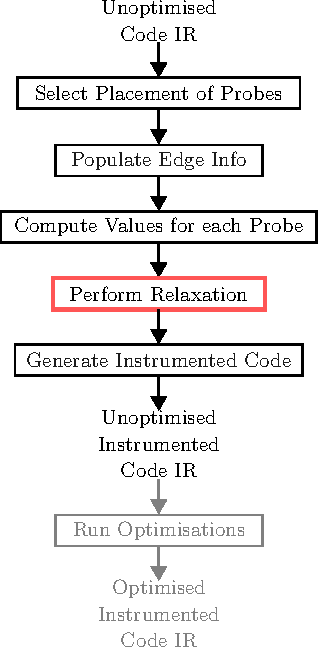
\includegraphics[scale=0.9]{figs/relax-instr-diagram.pdf}
  \caption{Diagram.}
  \label{fig:relax-instr-diagram}
\end{figure}

%\begin{figure*}[htb]
%    \centering
%    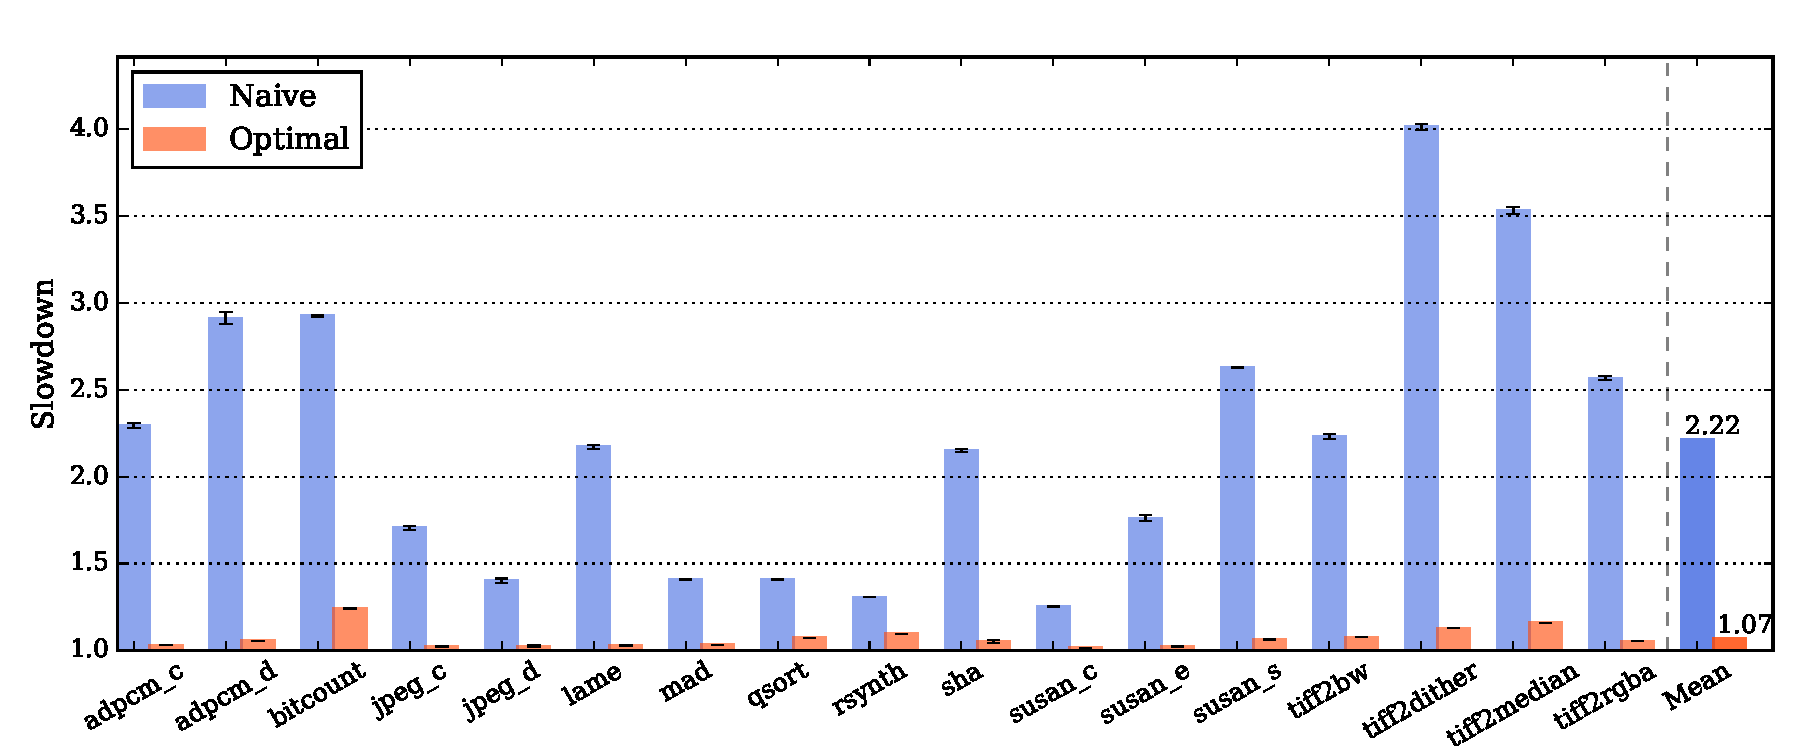
\includegraphics[width=\textwidth]{figs/overhead-O0.pdf}
%    \caption{Comparison between the naive and optimal instrumentation
%              with no compiler optimisation.}
%    \label{fig:overhead-O0}
%\end{figure*}

%Define an DAG of a CFG as a directed graph which may contain cycles if they have known constant trip counts.

The relaxed instrumentation performs a post-processing on the resulting instrumentation of the optimal algorithm.
The relaxation starts by extracting DAGs (directed acyclic graphs) from the CFG, as illustrated in Figure~\ref{fig:cfg-relax-example}.
The algorithm extracts all the subgraphs that represent a loop or the outer most region of the function.
These subgraphs are transformed into DAGs by ignoring the back edge and also by considering that any loop within the subgraph is never executed, i.e., only the headers of the inner loops are actually included into the DAG.
Figure~\ref{fig:cfg-relax-example} shows a CFG partitioned into two DAGs (consider only basic blocks and edges completely inside the yellow and green boundaries).
%
%LLVM has a Scalar Evolution Analysis which is used primarily to analyse expressions involving induction variables in loops~\cite{pop05}.
%An induction variable is a variable that is increased or decreased by a fixed amount on every iteration of a loop or is a linear function of another induction variable.
%
%This Scalar Evolution Analysis provides a way to compute \textit{small} constant trip counts (where \textit{small} is defined by a threshold).

\begin{figure}[h]
  \centering
  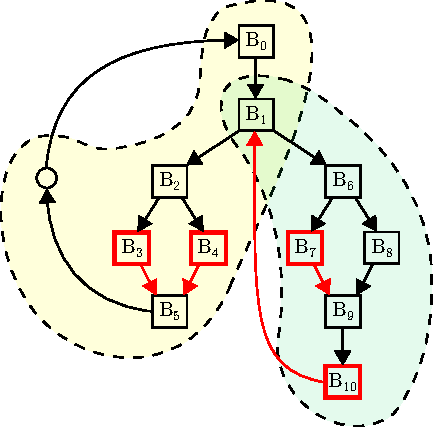
\includegraphics[scale=1]{figs/cfg-relax-example.pdf}
  \caption{Example of a CFG containing a loop and its decomposition into DAGs when applying the relaxation.
           The DAGs are the subgraphs within the dashed boundaries.}
  \label{fig:cfg-relax-example}
\end{figure}

For every DAG with a set of probes $\{P_0, P_1, \ldots, P_k\}$, we relax the instrumentation accuracy by selecting a subset of the probes to be removed, subject to the maximum allowed percentage error, $M$.

We model the relaxation as a 0-1 Knapsack problem:
\[
%\textrm{maximise } \sum_{i=0}^{k} f(I_i)c(I_i)x_i
\textrm{maximise } \sum_{i=0}^{k} f(P_i)x_i
\]
\[
\textrm{subject to } \sum_{i=0}^{k} \varepsilon(P_i)x_i \leq M \textrm{ and } x_i\in\{0,1\}
\]
%$c(I_i)$ is the relative overhead of the instrumentation on the instrumented basic block,
where $f(P_i)$ is the execution frequency of the instrumented basic block $P_i$, $\varepsilon(P_i)$ is the percentage error of removing probe $P_i$ relative to the minimum work value possible to compute in the DAG, and $x_i$ denotes the probes selected for removal.
Because the percentage error is computed based on the path with the minimum amount of work, $\varepsilon(P_i)$ represents the maximum error possible that would be incurred when removing probe $P_i$.
Furthermore, by constraining the percentage error of every DAG below a given threshold we guarantee that the final error of the relaxation will always be bounded by the threshold.

Let $n_i$ be the number of times a given DAG $i$ is executed, $r_i$ be the relaxation (amount of work removed) in DAG $i$, and $m_i$ be its minimum amount of work.
Let $\frac{r_i}{m_i} \leq T$ for every $i$.
Therefore, we can model the overall error of the relaxation as:
\[
1 - \frac{n_1(m_1 - r_1) + n_2(m_2 - r_2) + \ldots + n_k(m_k - r_k) + c}{n_1m_1 + n_2m_2 + \ldots + n_km_k + c}
\]
That is,
%\begin{equation*}
\begin{gather*}
 1 - \frac{n_1m_1 + n_2m_2 + \ldots + n_km_k + c}{n_1m_1 + n_2m_2 + \ldots + n_km_k + c} + \frac{n_1r_1 + n_2r_2 + \ldots + n_kr_k}{n_1m_1 + n_2m_2 + \ldots + n_km_k + c} = \\
 \frac{n_1r_1 + n_2r_2 + \ldots + n_kr_k}{n_1m_1 + n_2m_2 + \ldots + n_km_k + c}
\end{gather*}
%\end{equation*}
If $\frac{r_j}{m_j}$ is the maximum ratio $\frac{r_i}{m_i}$ for every $i$, then
\begin{equation*}
\begin{aligned}
 \frac{n_1r_1 + n_2r_2 + \ldots + n_kr_k}{n_1m_1 + n_2m_2 + \ldots + n_km_k + c} &\leq\\
 \frac{n_1r_j + n_2r_j + \ldots + n_kr_j}{n_1m_j + n_2m_j + \ldots + n_km_j + c} &\leq\\
 \frac{n_1r_j + n_2r_j + \ldots + n_kr_j}{n_1m_j + n_2m_j + \ldots + n_km_j} & 
\end{aligned}
\end{equation*}
If $N = max\{n_i$ for every $i\}$, then
\begin{equation*}
\begin{aligned}
 \frac{n_1r_j + n_2r_j + \ldots + n_kr_j}{n_1m_j + n_2m_j + \ldots + n_km_j} &\leq\\
 \frac{Nr_j + Nr_j + \ldots + Nr_j}{Nm_j + Nm_j + \ldots + Nm_j} &\leq\\
 \frac{Nkr_j}{Nkm_j} = \frac{r_j}{m_j} &\leq T
\end{aligned}
\end{equation*}

While the optimal placement of probes tries to place probes in edges that are less likely to be executed, the relaxation focus on removing probes that are more likely to be executed.
The necessary block frequency information for optimising both the placement of probes can be acquired from profiles of previous executions of the program or by a static heuristic of the CFG during compilation.

For our experiments, we implemented two solvers for the 0-1 Knapsack problem:
the optimal brute-force solver;
the greedy heuristic based on sorting the items~\citep{dantzig57}.
We use the brute-force solver for DAGs with a small number of probes and the greedy heuristic when the number of probes is greater than a threshold.
Some of the benchmarks have DAGs with several hundreds of probes, which could result in a long compilation time.

\section{Whole Program Relaxation}

In some cases, the proposed relaxation can be very conservative, because it considers the static error of removing probe $P_i$ relative to the minimum work possible of a DAG, in order to be able to guarantee that the dynamic error will be bounded by a given threshold.
This conservatism can be overly restrictive in some cases, resulting in a negligible overhead reduction but also causing only negligible dynamic error to the work profiling.

In some cases, this overly restrictive conservatism may be unecessary.
For these cases, we propose an adapted version of the relaxation algorithm that operates on the whole program.
Traditionally, compilers optimisations are performed on the function-level, or at best on a per module basis.
Whole program optimisation (WPO) means that the compiler considers all compilation units of the program and optimises them using the combined knowledge of how they are used together.

%Traditionally, compilers optimise a program procedure by procedure, or at best compilation unit per compilation unit. Whole program optimisation (WPO) means that the compiler considers all compilation units that make up a program or library and optimises them using the combined knowledge of how they are used together in this particular case.
%Whole program optimization is the compiler optimization of a program using information about all the modules in the program. Normally, optimizations are performed on a per module, "compiland", basis; but this approach, while easier to write and test and less demanding of resources during the compilation itself, does not allow certainty about the safety of a number of optimizations such as aggressive inlining and thus cannot perform them even if they would actually turn out to be efficiency gains that do not change the semantics of the emitted object code.



\section{Other Possible Uses}

\textbf{Talk about how this instrumentation techniques (relaxation) could be applied to other profiling-based mechanism to estimate input sizes~\citep{zaparanuks12,coppa14}, namely \textit{read memory size}}
